\documentclass[11pt]{article}

\usepackage[a4paper,margin=1in]{geometry}
\usepackage{booktabs}
\usepackage{graphicx}
\usepackage{hyperref}
\graphicspath{{figures/}}

\title{FastXeBench: A Reproducible Benchmark and Fidelity Study of Edit-to-PDF Latency for XeLaTeX on Windows}
\author{Zirui Xu\\Nanjing Normal University\\\texttt{19230444@njnu.edu.cn}}
\date{}

\begin{document}
\maketitle

\begin{abstract}
FastXeBench is a reproducible benchmark study of edit-to-PDF latency for XeLaTeX on Windows. The harness uses a prime-plus-measure protocol so that incremental scenarios time only the post-edit build rather than a fresh build. Our formal core matrix covers four workloads, five scenarios, and three main configurations, producing 45 workload-scenario-config groups and 900 recorded runs. We report per-group medians, IQRs, and bootstrap 95\% confidence intervals, with corrected nonparametric comparisons deferred to the appendix. The results are workload-sensitive: \texttt{latexmk} reliably improves steady incremental edits, but it is not universally faster on clean builds or bibliography edits, while \texttt{minted} cache is the strongest safe optimization on code-heavy documents. All main-matrix runs preserve visual equality with the baseline. Two real-project-derived validation workloads reproduce the \texttt{latexmk} pattern, and a scoped Windows storage follow-up shows that the observed \texttt{C:} profile root is about 1.20x slower than the repository-local \texttt{D:} root. These results position FastXeBench as both a benchmark artifact and a practical guide for Windows-local XeLaTeX workflows.
\end{abstract}

\section{Introduction}
XeLaTeX users often optimize their local edit-compile loop without a reproducible method for comparing toolchain choices. Recent evidence that TeX outputs can vary across engines and distribution versions means that latency alone is not a sufficient optimization target; fidelity must be measured alongside speed \cite{tan2024tex}. FastXeBench targets that gap with a runnable benchmark harness centered on edit-to-PDF latency rather than fresh-build latency.

This paper makes four concrete contributions. First, it packages a Windows-local XeLaTeX benchmark artifact with explicit workload, scenario, and configuration boundaries. Second, it fixes the measurement target at edit-to-PDF latency through a prime-plus-measure protocol rather than a fresh-build proxy. Third, it treats output fidelity as a release gate by combining PDF hashes with page-level raster comparison. Fourth, it turns the resulting dataset into practical guidance: \texttt{latexmk} is a steady incremental default, \texttt{minted} cache is the strongest safe code-heavy optimization in the present matrix, and excluded configurations are kept explicit rather than folded into optimistic recommendations.

\section{Background and Positioning}
FastXeBench is positioned as a Windows-local benchmark and engineering study rather than a new compiler. The comparison space is grounded in existing TeX tooling: \texttt{latexmk} automates reruns and dependency tracking \cite{ctan-latexmk}, \texttt{fontspec} exposes the native-font path that makes XeLaTeX attractive on Windows \cite{ctan-fontspec}, \texttt{minted} adds a realistic cache-heavy code-highlighting workload \cite{ctan-minted}, \texttt{mylatexformat} represents preamble dumping \cite{ctan-mylatexformat}, PGF/TikZ covers figure-heavy workflows \cite{ctan-pgf}, and Tectonic provides a modern cached-engine comparison point \cite{tectonic-build}. The paper is also prepared with an arXiv-first submission path in mind, so current arXiv XeLaTeX and TeX Live constraints matter directly \cite{arxiv-texlive,arxiv-multilang}.

\section{Benchmark Design}
Protocol v0.2 uses prime-plus-measure semantics for incremental scenarios: a stable state is built in an isolated run directory, a controlled edit is applied, and only the second build is timed. The current formal core matrix covers four workloads, five scenarios, and three main-matrix configurations (\texttt{B0}, \texttt{B1}, and \texttt{B4}). The workload set intentionally spans text-and-math, CJK/native-font, TikZ, and code-heavy documents, with the native-font and code-heavy paths explicitly exercising \texttt{fontspec} and \texttt{minted} behavior \cite{ctan-fontspec,ctan-minted}. Synthetic workloads provide controlled comparisons, while second-batch follow-up datasets add two real-project-derived validations and one scoped Windows storage comparison.

\begin{table}[t]
\centering
\caption{Experimental setup for the formal core dataset.}
\label{tab:setup}
\small
\begin{tabular}{p{0.28\linewidth}p{0.66\linewidth}}
\toprule
Item & Value \\
\midrule
Host CPU & 12th Gen Intel(R) Core(TM) i7-12700H (14 cores / 20 threads) \\
Memory & 15.6 GiB physical RAM \\
OS & Microsoft Windows 11 Home (Chinese edition), version 10.0.26100 (build 26100) \\
Machine & ASUS TUF Gaming F15 FX507ZV4\_FX507ZV4 \\
Power plan & Balanced \\
Repository volume & D: NTFS fixed volume; Defender performance mode status 0 \\
Primary TeX engine & XeTeX 3.141592653-2.6-0.999997 (TeX Live 2025) \\
Automation & Latexmk, John Collins, 15 June 2025. Version 4.87; hyperfine 1.20.0 \\
Follow-up engine & tectonic 0.15.0 \\
PDF comparison & pdftoppm version 25.02.0 at 144 dpi plus per-page PNG SHA-256 \\
Font path & \texttt{ctexart} on the local Windows CJK path; R1 validation uses TeX Gyre Pagella, Heros, and Cursor. \\
Formal protocol & \texttt{v0.2-prime-measure}; 4 workloads, 5 scenarios, 3 main configurations \\
Runs per group & 3 warmups and 20 recorded runs for the formal core matrix \\
\bottomrule
\end{tabular}
\end{table}


All formal measurements use the single Windows-local host summarized in Table~\ref{tab:setup}. Each recorded run executes in an isolated directory under the dataset root. Scenario \texttt{S0} measures a clean build directly, while \texttt{S1}--\texttt{S4} first build a stable state, apply one controlled mutation, and then time only the post-edit rebuild. Reference PDFs are generated per workload/scenario pair and reused for fidelity comparisons.

Fidelity is checked in two stages. The harness first records a whole-file SHA-256 for the candidate PDF and its workload/scenario reference. It then rasterizes both PDFs with \texttt{pdftoppm -png -r 144} and compares per-page PNG hashes. If any page hash differs, the run is marked \texttt{visual\_equal = false} and the changed page indices are recorded together with diagnostic diff images. In the present paper, \texttt{binary\_equal} is retained as a secondary indicator only; the main fidelity gate is \texttt{visual\_equal}.

Primary statistical summaries use group medians, IQRs, and 95\% bootstrap confidence intervals computed from the recorded wall-clock latencies. Appendix Table~\ref{tab:appendix-stats} adds Holm-corrected two-sided Wilcoxon signed-rank tests for the non-baseline configurations. Because the current artifact records repeated runs rather than an explicit cross-configuration pairing ID, these appendix tests pair runs by within-group recorded order after sorting \texttt{run\_id}; we therefore treat them as supporting evidence rather than stronger than the descriptive summaries themselves.

\section{Acceleration Techniques}
The current harness includes a direct XeLaTeX baseline, \texttt{latexmk} automation \cite{ctan-latexmk}, \texttt{minted} cache reuse \cite{ctan-minted}, a negative XeLaTeX-plus-\texttt{mylatexformat} compatibility case \cite{ctan-mylatexformat}, TikZ externalization as an appendix-only negative result rooted in PGF/TikZ workflows \cite{ctan-pgf}, and a Tectonic comparison that is retained as a development-only reference because of persistent fidelity differences \cite{tectonic-build}.

\section{Results}
The formal core dataset contains 45 workload-scenario-config groups and 900 recorded runs. All recorded runs succeeded, and every main-matrix row currently preserves visual equality with the baseline. This means the primary conclusions are driven by steady-state latency rather than speed-versus-fidelity trade-offs inside the core matrix. Table~\ref{tab:formal-rollup} compresses the main matrix, while Appendix Table~\ref{tab:appendix-stats} reports the per-group medians, IQRs, bootstrap confidence intervals, and corrected nonparametric tests.

Figure~\ref{fig:speedup-heatmap} shows that the main result is workload-sensitive rather than uniform. For the W1 text+math and W2 CJK+font workloads, \texttt{latexmk} reduces the S1, S3, and S4 edit latencies from about 7.1 seconds to about 4.0 seconds, yielding roughly 1.76x speedups, but it is slower than the baseline on clean builds and bibliography edits. For W4 TikZ, \texttt{latexmk} is close to neutral on clean builds and bibliography edits, while reducing text, figure, and preamble edits from about 10.1 seconds to about 4.0 seconds, for about 2.50x speedups. For W5 minted, \texttt{latexmk} lowers clean builds from about 43.1 seconds to about 38.0 seconds, and lowers S1, S3, and S4 to about 14.0 seconds, for about 3.07x speedups.

\begin{table}[t]
\centering
\caption{Formal core rollup for non-baseline configurations. Incremental latency is the median over S1, S3, and S4.}
\label{tab:formal-rollup}
\resizebox{\linewidth}{!}{%
\begin{tabular}{llrrrrrr}
\toprule
Workload & Config & Clean (s) & Clean $\times$ & Bib (s) & Bib $\times$ & Incremental (s) & Incremental $\times$ \\
\midrule
W1 Text+Math & B1 latexmk & 8.02 & 0.88 & 8.02 & 0.88 & 4.02 & 1.76 \\
W2 CJK+Font & B1 latexmk & 9.02 & 0.78 & 9.02 & 0.78 & 4.02 & 1.76 \\
W4 TikZ & B1 latexmk & 10.02 & 1.01 & 10.02 & 1.01 & 4.02 & 2.51 \\
W5 Minted & B1 latexmk & 38.02 & 1.13 & 38.01 & 1.13 & 14.01 & 3.07 \\
W5 Minted & B4 minted cache & 19.02 & 2.26 & 16.02 & 2.69 & 6.01 & 7.16 \\
\bottomrule
\end{tabular}
}
\end{table}


\begin{figure}[t]
\centering
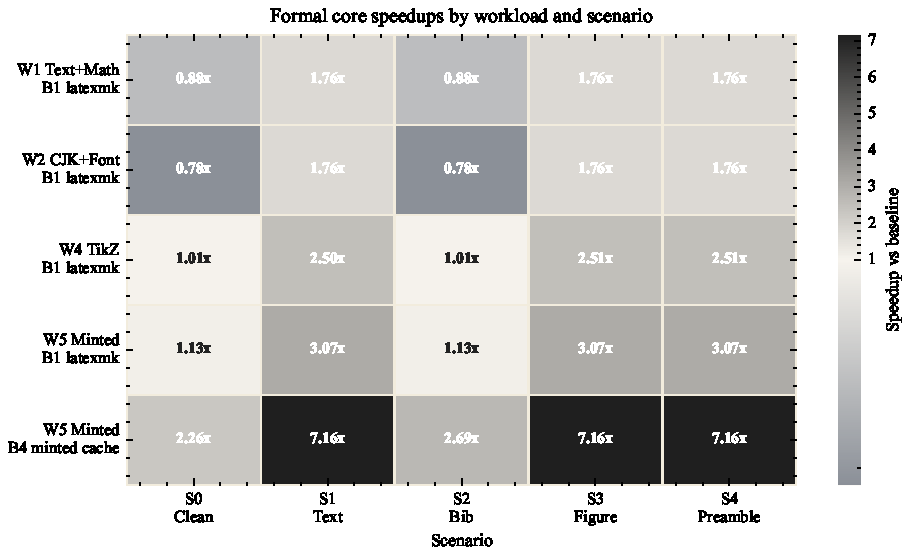
\includegraphics[width=\linewidth]{formal_speedup_heatmap.pdf}
\caption{Formal speedup matrix for the non-baseline configurations. Values above 1.0 indicate lower latency than the XeLaTeX baseline.}
\label{fig:speedup-heatmap}
\end{figure}

\begin{figure}[t]
\centering
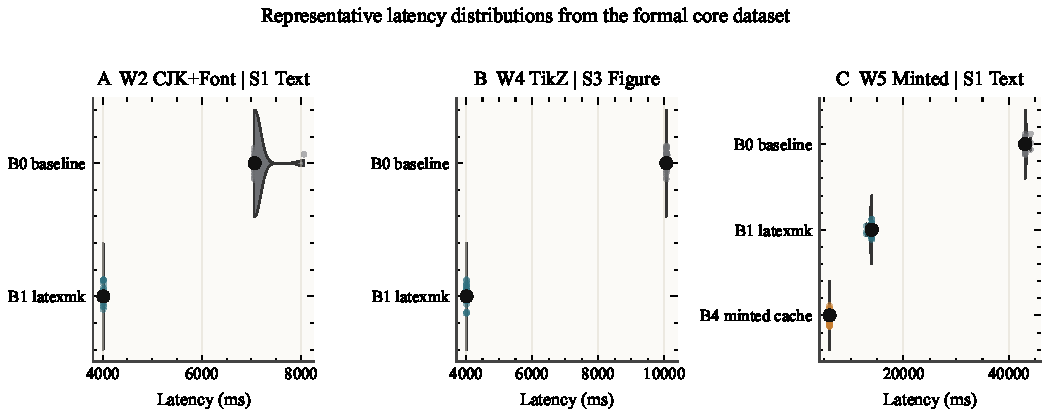
\includegraphics[width=\linewidth]{formal_latency_panels.pdf}
\caption{Representative per-run latency distributions. Panel A shows \texttt{W2} text edits, panel B shows \texttt{W4} figure edits, and panel C shows \texttt{W5} text edits with both \texttt{latexmk} and \texttt{minted} cache.}
\label{fig:latency-panels}
\end{figure}

\texttt{minted} cache is the strongest stable optimization in the current core matrix. On W5 minted, it reduces clean-build latency to about 19.0 seconds (2.26x over baseline), reduces bibliography edits to about 16.0 seconds (2.69x), and reduces text, figure, and preamble edits to about 6.0 seconds (about 7.16x), while preserving visual equality in all recorded runs. Figure~\ref{fig:latency-panels} makes this separation visible at the run level rather than only at the level of group medians.

Appendix Table~\ref{tab:appendix-stats} shows that these group differences remain statistically distinguishable after Holm correction. That result should be read carefully: corrected significance does not imply universal speedup, because several \texttt{B1} clean-build and bibliography cells are significantly slower than the direct XeLaTeX baseline even while the incremental cells remain significantly faster.

The second-batch follow-up results support the same interpretation. In the external validation dataset, two real-project-derived workloads, R1 (a \texttt{fontspec}-oriented example) and R2 (a \texttt{pgfplots}-oriented example), reproduce the \texttt{latexmk} pattern seen in the synthetic matrix: clean builds and bibliography edits are slower than the direct XeLaTeX baseline at about 0.78x baseline speed, while incremental edits still improve by about 1.76x, again with full visual equality. In the B7 storage dataset, the passive Windows storage comparison between \texttt{d\_repo\_ntfs} and \texttt{c\_profile\_ntfs} preserves visual equality in all nine groups, but the \texttt{c\_profile\_ntfs} root is slower overall, with a median latency ratio of about 1.20x relative to the repository-local \texttt{D:} root. Appendix Tables~\ref{tab:external-validation} and \ref{tab:b7-storage} summarize these follow-up datasets directly.

\begin{figure}[t]
\centering
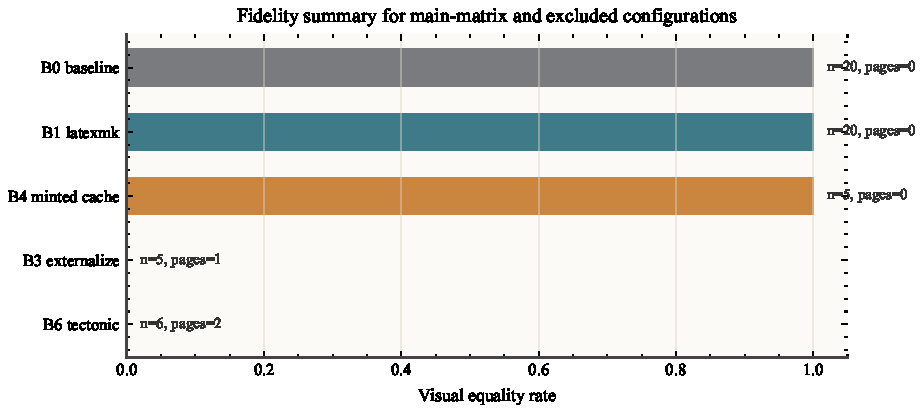
\includegraphics[width=0.92\linewidth]{formal_fidelity_summary.pdf}
\caption{Visual-equality summary for the main-matrix configurations and the excluded \texttt{B3}/\texttt{B6} diagnostic paths. The core matrix remains fully visually equal, while triage reproduces persistent fidelity failures for the excluded configurations.}
\label{fig:fidelity-summary}
\end{figure}

\section{Threats to Validity}
The current artifact still runs on a single Windows host, so the reported latency distributions inevitably include host-specific effects such as storage layout, antivirus state, and local font availability. The workload mix also remains partly synthetic even after the two real-project-derived validation workloads were added, which means the benchmark is stronger as a controlled comparative study than as a claim about every class of TeX project. The storage follow-up is especially scoped: Dev Drive is intended as a dedicated Windows developer volume \cite{ms-devdrive}, but the current environment does not permit a full privileged Dev Drive provisioning or direct performance-mode manipulation. The benchmark therefore reports a Windows-local storage-root comparison under the observed system state, not a universal claim about all Dev Drive configurations. Finally, the current paper emphasizes descriptive results and reproducible artifacts; the appendix-level Wilcoxon analysis is informative, but it depends on recorded-order pairing rather than an explicit synchronized cross-config run identifier.

\section{Conclusion}
The current evidence supports a conservative recommendation set. For steady incremental writing loops, \texttt{latexmk} is the default win, but its gains are workload- and scenario-dependent rather than universal. For code-heavy documents, \texttt{minted} cache is the strongest safe optimization in the present matrix. Fidelity should remain a release gate, not an afterthought, because configuration choices that look attractive from latency alone can still produce visible output differences. This leaves FastXeBench in a useful position for an arXiv-first release: the benchmark results are stable, the excluded configurations are explicitly scoped, and the repository now supports both reruns and paper regeneration from the recorded datasets.

\section{Artifact Availability}
The benchmark workloads, orchestration scripts, clean dataset layout, and environment metadata are publicly available at \url{https://github.com/handsomeZR-netizen/fastxebench}. The repository is intended to expose the benchmark harness, paper sources, analysis scripts, and compact result artifacts needed to regenerate the figures and tables, while larger raw datasets may be distributed as release assets. The current submission path is intentionally arXiv-first. arXiv currently supports TeX Live 2023 and 2025, with 2025 as the default, and provides specific XeLaTeX guidance for filename-based \texttt{fontspec} loading and minted-v3 cache generation \cite{arxiv-texlive}. If a multilingual version is prepared later, the English version should appear first \cite{arxiv-multilang}. To reduce packaging risk, the repository also includes a local dry-run checklist and isolated submission-bundle script.

\appendix
\section{Appendix Statistics}
\begin{table}[p]
\centering
\caption{Appendix statistics for the non-baseline main-matrix configurations. IQR is reported as $[Q_1, Q_3]$, CI is the 95\% bootstrap interval for the group median, and Holm-adjusted $p$ values come from two-sided Wilcoxon signed-rank tests that pair runs by within-group recorded order after sorting by \texttt{run\_id}.}
\label{tab:appendix-stats}
\small
\resizebox{\linewidth}{!}{%
\begin{tabular}{lllrrrrr}
\toprule
Workload & Scenario & Config & Median (s) & IQR (s) & 95\% CI (s) & Speedup & Holm $p$ \\
\midrule
W1 Text+Math & S0 clean & B1 latexmk & 8.02 & [8.01, 8.02] & [8.01, 8.02] & 0.88 & <0.001 \\
W1 Text+Math & S1 text & B1 latexmk & 4.02 & [4.01, 4.02] & [4.01, 4.02] & 1.76 & <0.001 \\
W1 Text+Math & S2 bib & B1 latexmk & 8.02 & [8.01, 8.02] & [8.01, 8.02] & 0.88 & <0.001 \\
W1 Text+Math & S3 figure & B1 latexmk & 4.02 & [4.01, 4.02] & [4.01, 4.02] & 1.76 & <0.001 \\
W1 Text+Math & S4 preamble & B1 latexmk & 4.02 & [4.01, 4.02] & [4.01, 4.02] & 1.76 & <0.001 \\
W2 CJK+Font & S0 clean & B1 latexmk & 9.02 & [9.01, 9.02] & [9.01, 9.02] & 0.78 & <0.001 \\
W2 CJK+Font & S1 text & B1 latexmk & 4.02 & [4.01, 4.02] & [4.01, 4.02] & 1.76 & <0.001 \\
W2 CJK+Font & S2 bib & B1 latexmk & 9.02 & [9.01, 9.02] & [9.01, 9.02] & 0.78 & <0.001 \\
W2 CJK+Font & S3 figure & B1 latexmk & 4.01 & [4.01, 4.02] & [4.01, 4.02] & 1.76 & <0.001 \\
W2 CJK+Font & S4 preamble & B1 latexmk & 4.02 & [4.01, 4.02] & [4.01, 4.02] & 1.76 & <0.001 \\
W4 TikZ & S0 clean & B1 latexmk & 10.02 & [10.01, 10.02] & [10.01, 10.02] & 1.01 & <0.001 \\
W4 TikZ & S1 text & B1 latexmk & 4.02 & [4.02, 4.02] & [4.02, 4.02] & 2.50 & <0.001 \\
W4 TikZ & S2 bib & B1 latexmk & 10.02 & [10.01, 10.02] & [10.02, 10.02] & 1.01 & <0.001 \\
W4 TikZ & S3 figure & B1 latexmk & 4.02 & [4.01, 4.02] & [4.02, 4.02] & 2.51 & <0.001 \\
W4 TikZ & S4 preamble & B1 latexmk & 4.01 & [4.01, 4.02] & [4.01, 4.02] & 2.51 & <0.001 \\
W5 Minted & S0 clean & B1 latexmk & 38.02 & [38.01, 38.02] & [38.01, 38.02] & 1.13 & <0.001 \\
W5 Minted & S0 clean & B4 minted cache & 19.02 & [19.01, 19.02] & [19.01, 19.02] & 2.26 & <0.001 \\
W5 Minted & S1 text & B1 latexmk & 14.02 & [14.01, 14.02] & [14.01, 14.02] & 3.07 & <0.001 \\
W5 Minted & S1 text & B4 minted cache & 6.02 & [6.01, 6.02] & [6.01, 6.02] & 7.16 & <0.001 \\
W5 Minted & S2 bib & B1 latexmk & 38.01 & [38.01, 38.02] & [38.01, 38.02] & 1.13 & <0.001 \\
W5 Minted & S2 bib & B4 minted cache & 16.02 & [16.01, 16.02] & [16.01, 16.02] & 2.69 & <0.001 \\
W5 Minted & S3 figure & B1 latexmk & 14.01 & [13.76, 14.01] & [14.01, 14.01] & 3.07 & <0.001 \\
W5 Minted & S3 figure & B4 minted cache & 6.01 & [6.01, 6.02] & [6.01, 6.01] & 7.16 & <0.001 \\
W5 Minted & S4 preamble & B1 latexmk & 14.01 & [14.01, 14.02] & [14.01, 14.02] & 3.07 & <0.001 \\
W5 Minted & S4 preamble & B4 minted cache & 6.01 & [6.01, 6.02] & [6.01, 6.02] & 7.16 & <0.001 \\
\bottomrule
\end{tabular}
}
\end{table}


\begin{table}[t]
\centering
\caption{External validation rollup for the two real-project-derived workloads.}
\label{tab:external-validation}
\begin{tabular}{lrrrr}
\toprule
Workload & Clean $\times$ & Bib $\times$ & Incremental $\times$ & Visual eq. \\
\midrule
R1 fontspec & 0.78 & 0.78 & 1.76 & 1.00 \\
R2 pgfplots & 0.79 & 0.78 & 1.76 & 1.00 \\
\bottomrule
\end{tabular}
\end{table}


\begin{table}[t]
\centering
\caption{Scoped Windows storage follow-up. The baseline mode is the repository-local \texttt{D:} root.}
\label{tab:b7-storage}
\begin{tabular}{lrrrr}
\toprule
Mode & Groups & Volume & Median ratio & Visual eq. \\
\midrule
d\_repo\_ntfs & 9 & \texttt{D:/NTFS} & 1.00 & 1.00 \\
c\_profile\_ntfs & 9 & \texttt{C:/NTFS} & 1.20 & 1.00 \\
\bottomrule
\end{tabular}
\end{table}


\section{Excluded Configurations and Scoped Follow-up}
\texttt{B2} remains a compatibility-limited XeLaTeX negative result tied to the \texttt{mylatexformat} path \cite{ctan-mylatexformat}. \texttt{B3} delivered speedups on TikZ-heavy cases but produced persistent visual differences, so it is retained as an appendix-only negative result rather than a recommendation. \texttt{B6} remains development-only: Tectonic provides a useful cached-engine comparison point \cite{tectonic-build}, but its output differences were stable enough in triage to keep it out of the main matrix. \texttt{B7} should be read as a scoped Windows storage-root comparison rather than a complete Dev Drive experiment, because the current environment can observe Microsoft Defender and volume metadata but cannot exercise the full privileged Dev Drive path \cite{ms-devdrive}.

\bibliographystyle{plain}
\bibliography{refs}

\end{document}
